%%%%%%%%%%%%%%%%%%%%%%%%%%%%%%%%%%%%%%%%%%%%%%%%%%%%%%%%%%%%%%%%%%%%%%%%%%%%%%%%%%%%%%%%%%%%%%%%%%%%%%%%%%%%%%%%%%%%%%%%%%%%%%%%%%%%%%%%%%%%%%%%%%%%%%%%%%%%%%%%%%%%%%%%%%%%%%%%%%%%%%%%%%%%
% Written By Michael Brodskiy
% Class: AP Chemistry
% Professor: J. Morgan
%%%%%%%%%%%%%%%%%%%%%%%%%%%%%%%%%%%%%%%%%%%%%%%%%%%%%%%%%%%%%%%%%%%%%%%%%%%%%%%%%%%%%%%%%%%%%%%%%%%%%%%%%%%%%%%%%%%%%%%%%%%%%%%%%%%%%%%%%%%%%%%%%%%%%%%%%%%%%%%%%%%%%%%%%%%%%%%%%%%%%%%%%%%%

\documentclass[12pt]{article} 
\usepackage{alphalph}
\usepackage[utf8]{inputenc}
\usepackage[russian,english]{babel}
\usepackage{titling}
\usepackage{amsmath}
\usepackage{graphicx}
\usepackage{enumitem}
\usepackage{amssymb}
\usepackage[super]{nth}
\usepackage{expl3}
\usepackage[version=4]{mhchem}
\usepackage{hpstatement}
\usepackage{rsphrase}
\usepackage{everysel}
\usepackage{ragged2e}
\usepackage{geometry}
\usepackage{fancyhdr}
\usepackage{cancel}
\usepackage{siunitx}
\usepackage{chemfig}
\geometry{top=1.0in,bottom=1.0in,left=1.0in,right=1.0in}
\newcommand{\subtitle}[1]{%
  \posttitle{%
    \par\end{center}
    \begin{center}\large#1\end{center}
    \vskip0.5em}%

}
\DeclareSIUnit\Molar{\textsc{m}}
\DeclareSIUnit\atm{\textsc{atm}}
\DeclareSIUnit\torr{\textsc{torr}}
\DeclareSIUnit\psi{\textsc{psi}}
\DeclareSIUnit\bar{\textsc{bar}}
\usepackage{hyperref}
\hypersetup{
colorlinks=true,
linkcolor=blue,
filecolor=magenta,      
urlcolor=blue,
citecolor=blue,
}

\urlstyle{same}


\title{Chapter 7 $-$ Covalent Bonds}
\date{\today}
\author{Michael Brodskiy\\ \small Instructor: Mr. Morgan}

% Mathematical Operations:

% Sum: $$\sum_{n=a}^{b} f(x) $$
% Integral: $$\int_{lower}^{upper} f(x) dx$$
% Limit: $$\lim_{x\to\infty} f(x)$$

\begin{document}

\maketitle

\begin{itemize}

  \item Lewis Structures:

    \begin{enumerate}

      \item Sum Valence Electrons

      \item Connect atoms with lines

      \item Arrange remaining \ce{e-} to satisfy octet rule

    \end{enumerate}

  \item Resonance $-$ Being able to draw more than one Lewis structure

  \item Halogens will almost never have double bonds

  \item Molecular Shapes:

    \begin{enumerate}

      \item Linear

        \begin{itemize}

          \item Bond angle equals $180^{\circ}$

          \item Usually non-polar

          \item Ex:

            \chemfig{\lewis{2:6:,O}=C=\lewis{2:6:,O}}

        \end{itemize}

      \item Triangular Planar

        \begin{itemize}

          \item Bond angle equals $120^{\circ}$

          \item Usually non-polar

          \item Ex:

            \vspace{5pt}
            \chemfig{B(=[6]F)(-[:-210]F)(-[:-330]F)}

        \end{itemize}

      \item Bent

        \begin{itemize}

          \item Bond angle equals $109.5^{\circ}$

          \item Appears as a linear, but bent

          \item Always polar

          \item Ex:

            \chemfig{\lewis{2:6:,O}(-[:-144.5]H)(-[:-35]H)}

        \end{itemize}

      \item Tri-Pyramid

        \begin{itemize}

          \item Bond angle equals $109.5^{\circ}$

          \item Appears as a three dimensional, triangular pyramid

          \item Always polar

          \item Ex:

            \chemfig{\lewis{2:,N}(-[6]H)(-[:-10]H)(-[:-170]H)}

        \end{itemize}

      \item Tetrahedral

        \begin{itemize}

          \item Bond angle equals $109.5^{\circ}$

          \item Appears as a three dimensional, square pyramid

          \item Usually non-polar

          \item Ex:

            \chemfig{C(-[0]H)(-[2]H)(-[4]H)(-[6]H)}

        \end{itemize}

    \end{enumerate}

  \item Expanded Octets: \ce{5e-} pairs

    \begin{enumerate}

      \item Tri-Bipyramid (5 atoms)

        \begin{enumerate}

          \item Usually non-polar

        \end{enumerate}

      \item Seesaw (4 atoms) 

        \begin{enumerate}

          \item Always polar

        \end{enumerate}

      \item T Shape (3 atoms)

        \begin{enumerate}

          \item Always polar

        \end{enumerate}

      \item Linear (2 atoms)

        \begin{enumerate}

          \item Usually non-polar

        \end{enumerate}

    \end{enumerate}

  \item Expanded Octets: \ce{6e-} pairs

    \begin{itemize}

      \item Octahedral (6 atoms)

        \begin{enumerate}

          \item Usually non-polar

        \end{enumerate}

      \item Square Pyramid (5 atoms)

        \begin{enumerate}

          \item Always polar

        \end{enumerate}

      \item Square Planar (4 atoms)

        \begin{enumerate}

          \item Usually non-polar

        \end{enumerate}

    \end{itemize}

  \item VESPR $-$ \ce{e-} pairs repel, and double and triple bonds count as one pair.

  \item Molecular Polarity $-$ The negative side is what repels branching atoms, while the branching atoms are attracted to the positive side.

  \item Exceptions $-$ \ce{NF3} has a bond angle of $102^{\circ}$, \ce{CF4} has a bond angle of $109.5^{\circ}$. This is because lone pairs repel more than bonding pairs.

  \item These types of graphs show the appropriate bond distance between two atoms:

    \begin{figure}[h]
      \centering
      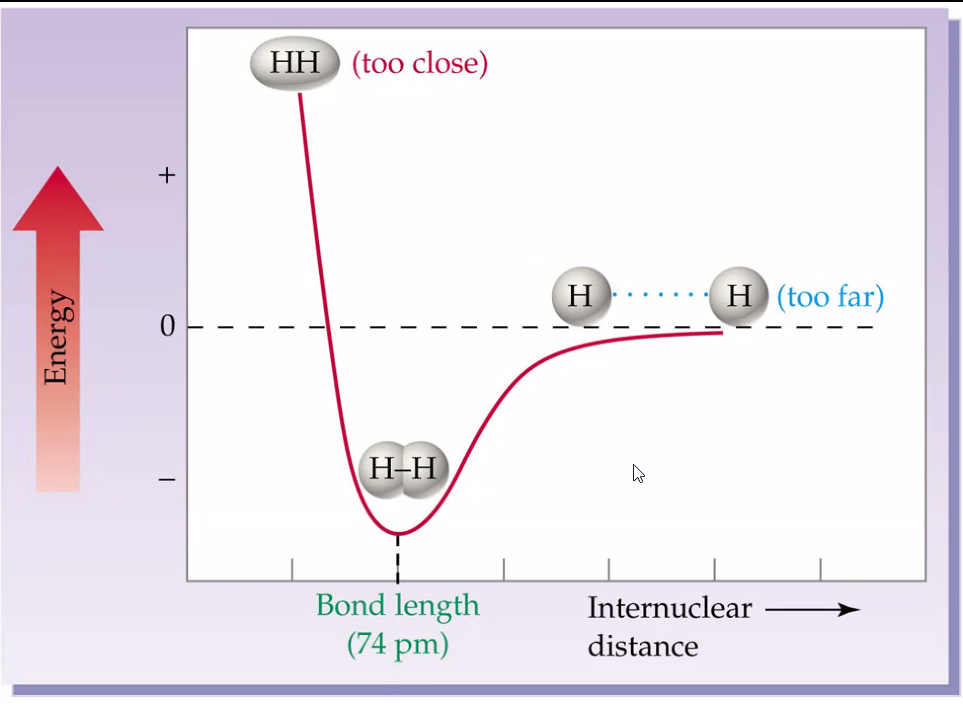
\includegraphics[width=.7\textwidth]{Figures/HappyGraph.png}
      \caption{Best Bonding Distance For \ce{H2}}
      \label{fig:1}
    \end{figure}

    \newpage
  \item The AP Exam will show a graph like the following and ask what is incorrect. Horizontal is determined by protons, while vertical is determined by size of the atom. In this case, \ce{F2} should be left of \ce{I2}

    \begin{figure}[h]
      \centering
      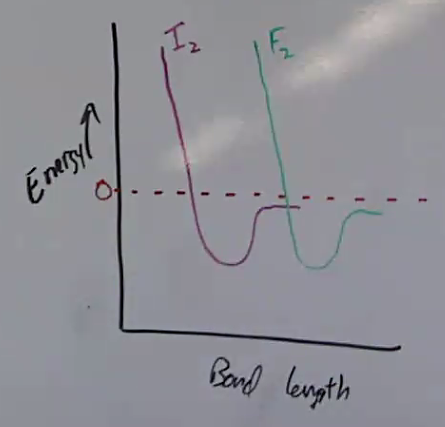
\includegraphics[width=.7\textwidth]{Figures/I2F2.png}
      \caption{Incorrect Energy Required to Break \ce{I2} and \ce{F2} Bonds}
      \label{fig:2}
    \end{figure}

\end{itemize}

\end{document}

